\documentclass[a4paper,12pt]{article}

%% Language and font encodings
\usepackage{polski}
\usepackage[utf8x]{inputenc}
\usepackage[T1]{fontenc}
\usepackage[table]{xcolor}
\usepackage{titling}
\usepackage{svg}
\usepackage[section]{placeins}
\usepackage{hyperref}
\usepackage{listings}
%% Sets page size and margins
\usepackage[a4paper,top=3cm,bottom=2cm,left=3cm,right=3cm,marginparwidth=1.75cm]{geometry}

%% Useful packages
%\usepackage{amsmath}
\usepackage{graphicx}
%\usepackage[colorinlistoftodos]{todonotes}
%\usepackage[colorlinks=true, allcolors=blue]{hyperref}

\title{Symulacja dziekanatu} 
\author{Marcin Skowron, Michał Kałduś}

\begin{document}



\begin{titlepage}
    \centering
    \vfill
    {\bfseries\Large
        Programowanie współbieżne i rozproszone\\

    }    
    \vfill
    
\includegraphics[width=4cm]{agh.jpg} 
    \vfill
    
     {\bfseries\Large
     	Symulacja dziekanatu \\ 
     Prowadzący: dr inż. Jacek Piwowarczyk \\
     Autorzy:Marcin Skowron i Michał Kałduś\\
    }  
    \vfill
\end{titlepage}


\tableofcontents

\newpage


\section{Cel programu}
	
Celem wykonanego przez nas programu była symulacja instytucji publicznej jaką jest dziekanat. Wykonany przez nas system odzwierciedla zachowania dziekanatu na Akademiku Górniczo Hutniczej w Krakowie na wydziale Elektrotechniki, Automatyki, Informatyki i Inżynierii Biomedycznej. Najważniejszym punktem wykonania projektu było zastosowanie mechanizmów współbieżności w celu zrealizowania poszczególnych zachowań symulowanego obiektu.











\section{Opis systemu}

 Pogram obejmuje symulację pracy 5 osób odpowiedzialnych za przyjmowanie studentów (panie z dziekanatu), pana dziekana, wyświetlacz przydzielający kolejne numery w kolejce dla petentów oraz samych studentów.
 Każdy z wyżej wymienionych elementów jest osobnym procesem w celu urealistycznienia zachowania.
 Dodatkowo napisany przez nas program jest bardzo mocno parametryzowalny.  Możemy ustawić jak szybko wykonuje się dana symulacja (przeskalowanie odpowiednio jednostki czasu) oraz z jaką częstotliwością przychodzą studenci. Ilość petentów jest też uzależniona od aktualnej godziny w systemie. Przebywająca osoba w dziekanacie może zostać na różne sposoby obsłużona między innymi:
 
 \begin{itemize}
 	\item poprawnie obsłużona
 	\item odesłana do dziekana
 	\item poproszona o przyjście innego dnia
 \end{itemize}
 
Kolejnym elementem programu jest to że każdy student po obsłużeni oraz w trakcie czekania w kolejce wyraża swoją opinie, którą może być:
 \begin{itemize}
	\item radość z poprawnego obsłużenia w dziekanacie
	\item narzekanie na przerwę w pracy obsługi dziekanatu
	\item poinformowanie o przymusie udania się do dziekana
	\item smutek z powodu nie załatwienia swojej sprawy
\end{itemize}

\section{Struktura logiczna}
Obrazki UML %%TODO

\section{Specyfikacja projektu}
	W celu zrealizowania warstwy widoku naszego projektu posłużyliśmy się biblioteką \nobreak \textbf{cecho} ze strony \url{https://github.com/mazenharake/cecho}, która adaptuje bibliotekę ncurses z języka C. 
	Aby ułatwić kompilacje i budowanie projektu użyliśmy narzędzia o nazwie: \textit{rebar}.
	W celu łatwego i szybkiego uruchamiania projektu stworzyliśmy skrypt uruchomieniowy \textit{run.escript}.
	
	W celu poprawnego uruchomienia aplikacji należy w terminalu wpisać dwie poniższe komendy.
	
	\textbf{UWAGA! Należy pamiętać o nadaniu odpowiednich praw tym dwóm plikom.}
	
	\begin{lstlisting}
	./rebar compile
	./run.escript
	\end{lstlisting}
	
	\newpage
	\section{Przykłady}
	
	\begin{figure}[!htb]
		\centering
		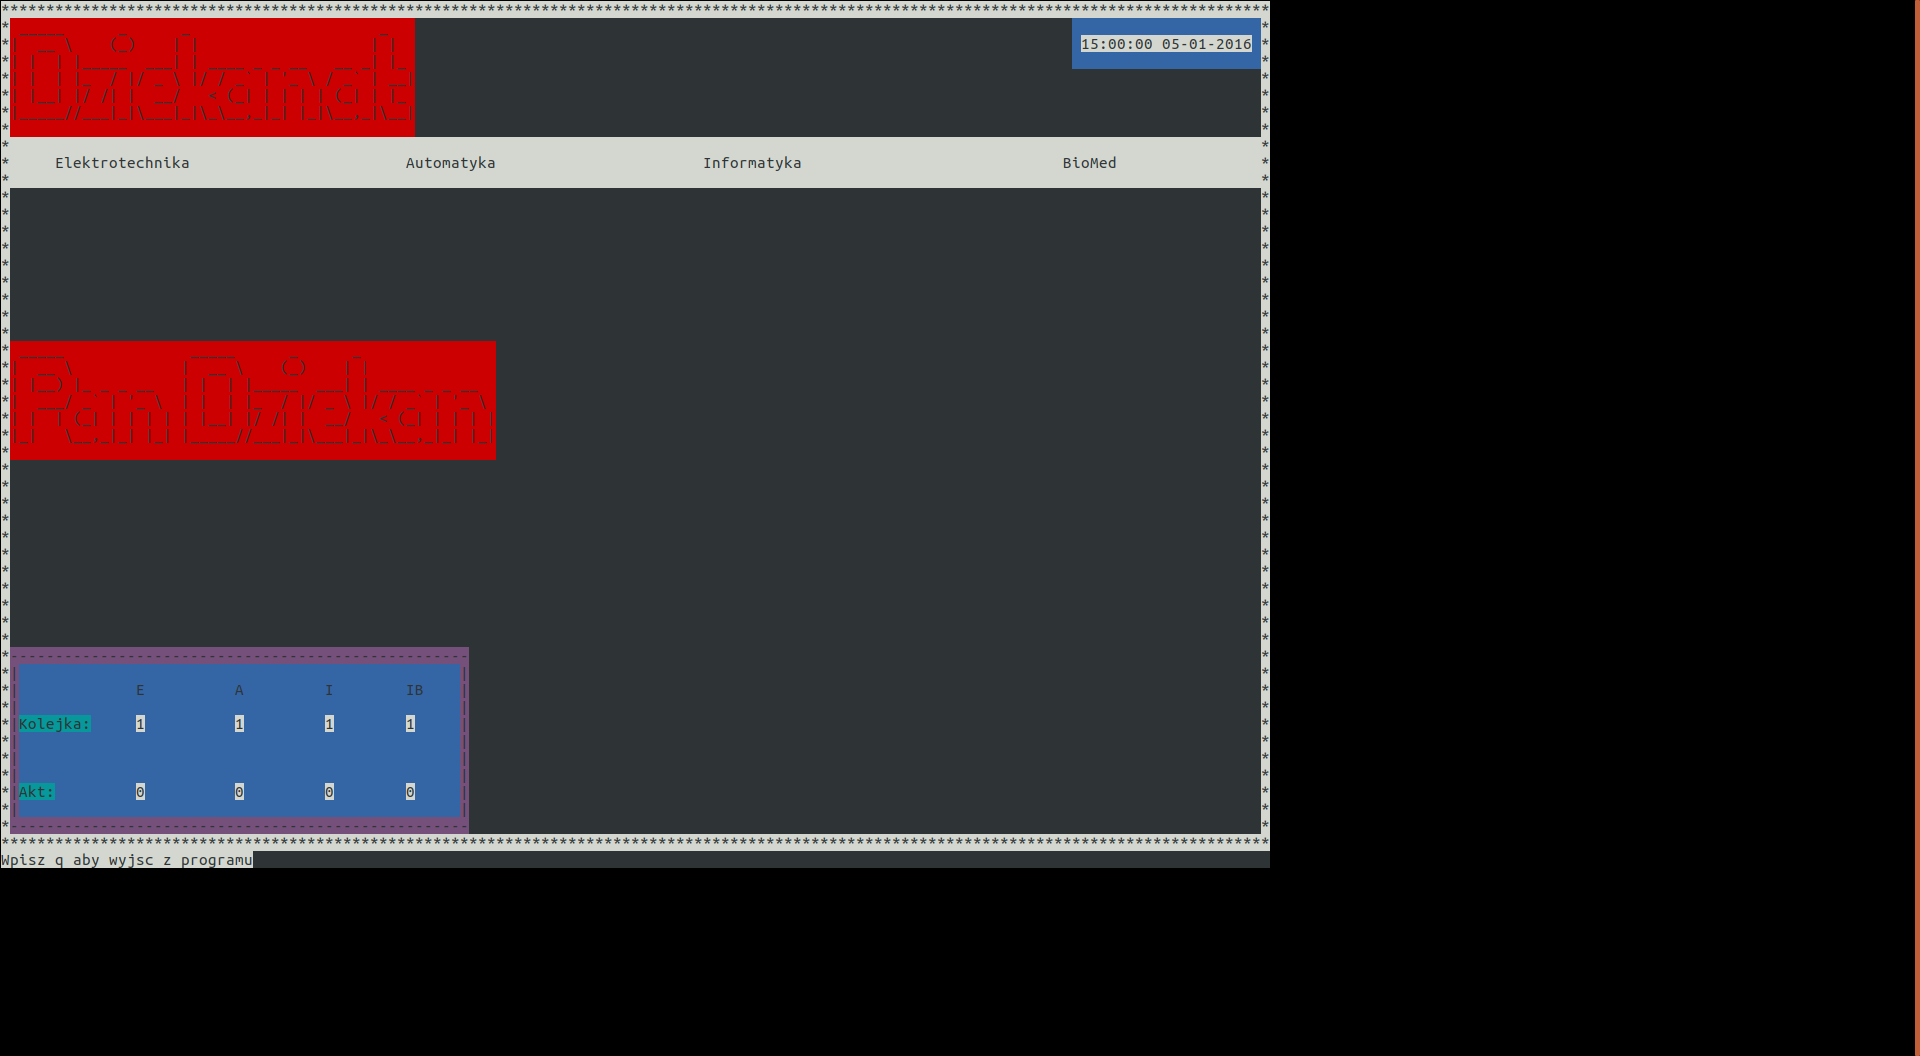
\includegraphics[width=1.1\linewidth]{terminal1}
		\caption{\label{fig:screen} Zrzut ekranu}
	\end{figure}

	\begin{figure}[!htb]
	\centering
	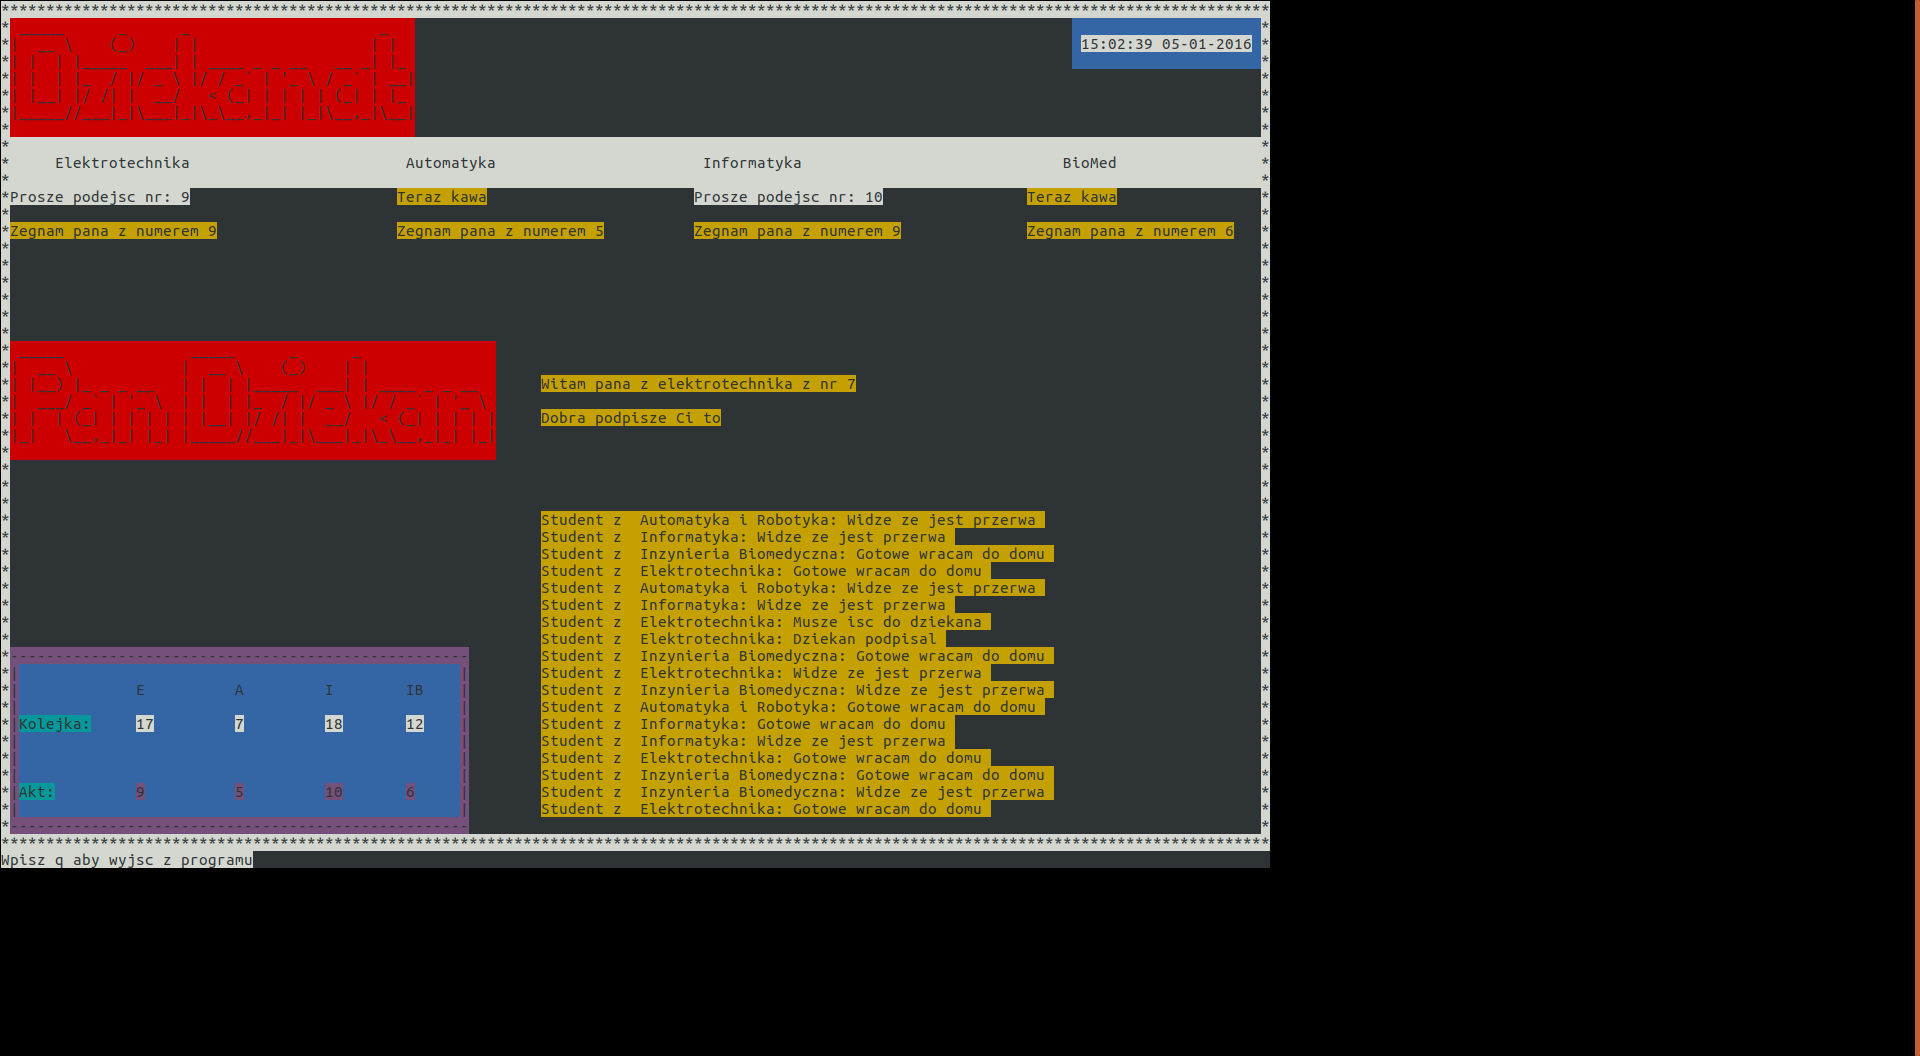
\includegraphics[width=1.1\linewidth]{terminal2}
	\caption{\label{fig:screen2} Zrzut ekranu}
\end{figure}
	

	\section{Rozszerzenia}
	
	Do programu można dodać możliwość wprowadzania nowych studentów ze standardowego wejścia w czasie trwania programu.
	
	Kolejną możliwością rozbudowania jest dodanie mechanizmu odesłania studenta, który ma przyjść do dziekanatu za określoną ilość czasu.
	
	Ciekawym rozszerzeniem programu mogłoby być dodanie mechanizmu odciążania bardziej obciążonych sekcji, przez sekcji, które nie mają aktualnie studentów w kolejce lub maja ich znacznie mniejszą ilość.
	
	Innym nieco bardziej skompilowanym sposobem ulepszenia projektu mogłoby być zmiana sposób prezentacji danych np.	zmienić aktualny terminal na okno przeglądarki internetowej

\end{document}